\documentclass[12pt,a4paper]{jsarticle}
\usepackage[dvipdfmx]{graphicx}
\usepackage[dvipdfmx]{color}
\usepackage{listings,jlisting}% to use japanese correctly, install jlistings.
\lstset{
  basicstyle={\small\ttfamily},
  identifierstyle={\small},
  commentstyle={\small\itshape\color{red}},
  keywordstyle={\small\bfseries\color{cyan}},
  ndkeywordstyle={\small},
  stringstyle={\small\color{blue}},
  frame={tb},
  breaklines=true,
  numbers=left,
  numberstyle={\scriptsize},
  stepnumber=1,
  numbersep=1zw,
  xrightmargin=0zw,
  xleftmargin=3zw,
  lineskip=-0.5ex
}
\lstdefinestyle{customCsh}{
  language={csh},
  numbers=none,
}
\lstdefinestyle{customRuby}{
  language={ruby},
  numbers=left,
}
\lstdefinestyle{customTex}{
  language={tex},
  numbers=none,
}
\lstdefinestyle{customJava}{
  language={java},
  numbers=left,
}
\begin{document}
\title{卒業論文\\ 
\vspace{4cm} RubyからMapleを呼び出す\\インターフェースライブラリ開発}
\author{ 関西学院大学 理工学部 情報科学科\\\\ 3528    村瀬 愛理}
\date{\vspace{3cm} 2017年  3月\\
\vspace{3cm} 指導教員  西谷 滋人 教授}
\maketitle
\setcounter{tocdepth}{4}
\tableofcontents

\section{概要}
西谷研究室では数値計算を用いた研究を行っている.その研究で度々使われるのが数式処理ソフトウェアの1つである
Mapleである.また,プログラミングにおいてはRubyを用いている.
Rubyは数値計算関連の環境設備が遅れているため,Rubyのみで高等な関数,
例えば,大きな素数を生成したり,最小公倍数を求めるなどの処理を行うのが難しい.また,扱える数値の桁数が
計算内容によっては足りないということも考えられる.
一方で,Ruby以外の数式処理ソフトウェアなどを立ち上げて,
別々に作業したり,慣れない別の言語を勉強し直したりするよりもRubyのみでプログラミングする方が,
開発速度の格段の向上が期待できる.
そこで本研究では,MapleをRuby上で呼び出し,Mapleに
高等な関数や桁数の大きな数値を用いた計算をさせて,
その結果をRubyが取得するインターフェースライブラリの開発を目的とする.


\section{第二章 序論}
\subsection{Mapleとは}
Mapleは,1980年にカナダ・ウォータールー大学で生まれた数式処理技術をコアテクノロジーとして持つ
科学・技術・工学・数学(STEM : Science, Technology, Engineering and Mathematics)に関する
統合的計算環境である[1].
特徴として,たくさんの数学関数が用意されていること,
大きな桁数の計算が可能であること,グラフの描画が簡単であり,かつ3次元のグラフの描画にも対応していることなどが挙げられる.
数式を入力するだけで簡単に解を得ることができることから,多くの場で用いられている.

\subsection{Rubyとは}
Rubyは,まつもとゆきひろ氏によって開発されたオブジェクト指向スクリプト言語である.
他にもテキスト処理に適した正規表現や高階関数,ガベージ・コレクションなどの特徴を持っている.
フリーソースソフトウェアであるため,誰でも自由に使用することが可能である.

\subsubsection{RubyとPython}
Pythonは,Rubyと同じオブジェクト指向のスプリクト言語である.この2つは
度々比較され,どちらが優れているのかを議論されてきた.2つのスプリクト言語の
決定的な違いは何を得意としているかである.RubyはWeb分野を得意とするのに対し,Pythonは
数値計算やビッグデータを得意としている.逆にRubyは数値計算には弱く,PythonはWeb分野には弱い.
もちろんこの議論に答えはなく,本来は自分が何を
目的としたプログラムを作るのかで使い分けるのが理想だろう.しかし,Rubyを使い慣れている
人が数値計算をするためだけにPythonを勉強し直すよりも,Ruby上で数値計算ができる方が良いのは
明らかである.


\section{手法}
\subsection{Mapleとの通信手法}
Mapleは一般的に,グラフや数式の綺麗な出力や,数式の入力を初心者が直感的におこなえるようにJavaで作られたGUIを使って実行する.それとは別にcommand lineで実行される計算エンジン部が用意されている.そこで,開発するRubyライブラリでは,このエンジンに直接働きかけて操作する.Rubyで外部コマンドを実行するgem libraryのsystemuを使って,出力を得るようにしている.Ruby codeで要求コードを受け取った場合,そのコードをtmp.mwに書き込む.それをMapleで実行し,結果をテキストファイルで受けとることで出力を得る.

\subsection{Maple関数の類型化}
今回,数多く存在するMapleの数学関数の中から整数論と行列に関するものを選抜し実装した.
実装した整数論に関する関数の役割と入出力を表\ref{table:one}に示した.また,
行列に関する関数の役割と入出力を表\ref{table:two}に示した.

\begin{table}[htbp]\begin{center}
\caption{実装した整数論に関する関数の役割と入出力.}
\label{table:one}
\begin{tabular}{lllll}
\hline
関数名  &振る舞い  &入力型  &出力型  \\ \hline
nextprime  &次の素数を求める  &int  &int  \\
lcm  &最小公倍数  &int, int  &int  \\
gcd  &最大公約数  &int, int  &int  \\
rand  &乱数生成  &int  &int  \\
isprime  &素数判定  &int  &boolean  \\
ifactor  &素因数分解  &int  &string  \\
mod  &剰余  &int, int  &int  \\
\hline
\end{tabular}
\label{default}
\end{center}\end{table}
%for inserting separate lines, use \hline, \cline{2-3} etc.

\begin{table}[htbp]\begin{center}
\caption{実装した行列に関する関数の役割と入出力.}
\label{table:two}
\begin{tabular}{lllll}
\hline
関数名  &振る舞い  &入力型  &出力型  \\ \hline
importmatrix  &textファイルから  &string, string  &int  \\
 &行列を読み込む  & \\
matrix  &行列生成  &int, int, int  &array  \\
matrixinverse  &逆行列  &array  &string  \\
determinant  &行列式の解  &array  &float  \\
trancepose  &転置行列  &array  &string  \\
eigenvectors  &固有値, 固有ベクトル  &array  &string  \\
\hline
\end{tabular}
\label{default}
\end{center}\end{table}
%for inserting separate lines, use \hline, \cline{2-3} etc.

\newpage

\subsection{出力の切り替え}
Mapleから受け取ったままの出力は,値の前にスペースがたくさん入っていることや,出力が String 型であることから,その数値を使って計算をするようにプログラミングしていた場合に支障をきたす.このため,関数ごとに正しい型で出力できるようにwrapperを作る.
例えば,int 型で出力が欲しいものはexecをexec\_iから呼び出すことで対応する.このようにbooleanやfloatといった出力型に応じて,exec\_b,exec\_fのように関数を増やしていく.


\section{実装}
\subsection{maplerubyの基本動作}
入力された値の次の素数を出力するnextprimeを用いて説明する.

\begin{figure}[htbp]\begin{center}
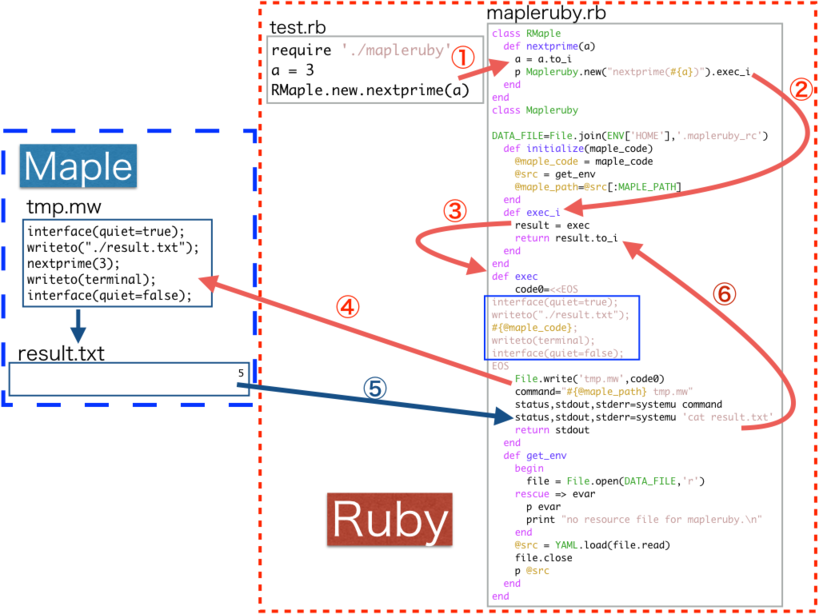
\includegraphics[width=10cm,bb= 0 0 737 553]{../figs/./mapleruby_eringi.003.png}
\caption{maplerubyの基本動作.}
\label{default}\end{center}\end{figure}
\begin{enumerate}
\item maplerubyをrequireした上で使いたい関数を使う.RMaple.new.hogehogeのhogehogeに使いたい関数名を入れる.今回はnextprimeで説明を進める.
\item RMapleクラス内のnextprime関数が呼び出され,aに3が入る.この時nextprimeは入力された値がint型になるように関数内でto\_iしてある.その後,Maplerubyクラスのexec\_i関数へ"nextprime(3)"が出力される.この出力された文字列がそのままMapleでの計算に使われる.
\item 出力された文字列をさらにexec関数へ出力する.
\item 青四角内の内容をMapleへと出力する.この時\verb|#{@maple_code};|となっている部分に先ほどの"nextprime(3)"が入る.青四角の内容がMapleに出力され実行されることで得られた答えがresult.txtに出力されるようになっている.
\item result.txtに出力された内容をRuby側で受け取り,exec\_iに再び返す.
\item 返された値をto\_iすることでint型に直して解を出力する.
\end{enumerate}
\subsection{出力の切り替えの実装例}
先ほどと同様にnextprimeを例に挙げるとexec\_iは,execでmapleに式を送った後mapleから受け取った値をto\_iし,int型にしてから返すようになっている.もし使われた関数が素数判定をtrue/falseで出力するisprimeだった場合は,出力はboolean型が好ましいため受け取った値をboolean型にするexec\_bを用いている.このように整数論に関する関数は,出力に応じてint型で解を得たい場合はexec\_i,float型ならexec\_f,string型ならexec\_sとすることで切り替えられるようになっている.

一方で,行列の場合は出力に切り替えについて例外が存在する.なぜなら,MapleのCUI版は行列の表現が図2のように独自のもので,それがresult.txtを通してRubyに出力されるからだ.
例えば,行列を生成する関数matrixは以下のように解を出力する.

\begin{figure}[htbp]\begin{center}
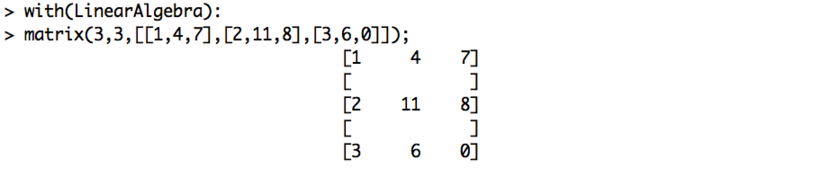
\includegraphics[width=10cm,bb= 0 0 737 553]{../figs/./mapleruby_eringi.exmatrix.png}
\caption{MapleCUI版での行列の表示.}
\label{default}\end{center}\end{figure}
この空白部分には半角スペースや改行が入っている上,余分な括弧が付いている.この関数を使う際に行列を生成して出力するだけなら問題ないが計算に数値を使う場合Rubyの方で都合の良い出力型に変える必要がある.そのためのwrapperを考える必要がある.そこで,int型の要素を持つlistlist構造で出力されるのが最も良いと考えた.今回実装した行列の関数の多くは,listlist構造のものをMapleのconvertというlistlist構造からMaple内で扱う行列の形に変換できる関数も一緒にRubyからMapleに送るようにしているためである.行列生成した後理想の型で値を得るためには,いらない記号や空白を取り除き要素をint型にする必要があった.図3はmatrixを実装した後,exec\_m(b)というwrapperを作ってみた際に生まれた失敗である.

\begin{figure}[htbp]\begin{center}
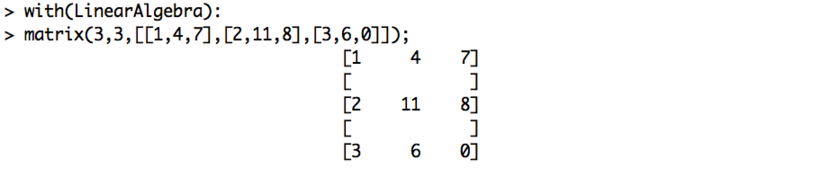
\includegraphics[width=10cm,bb= 0 0 737 553]{../figs/./mapleruby_eringi.004.png}
\caption{exec\_m(b)を実装した際の失敗例.}
\label{default}\end{center}\end{figure}
bには生成した行列の列の数が入る.実装する際に初めに考えたのが図3の左側のプログラムである.まずRubyのsplitメソッドを使って1文字ずつに分け,分けた要素全てをint型に変換する.空白はint型に変えた際0になるため,0になった空白部分をdelete\_ifメソッドを用いて削除し,最後にeach\_sliceメソッドを用いて1行目,2行目...と分けてそれぞれ配列に入れ,出力したかった行列と同じようなlistlist構造になるはずだった.しかし,listlist構造への変換はできていたが途中delete\_ifメソッドにより0を消してしまったため,行列の要素で0が含まれていた場合に行列の要素まで消えてしまった.しかも,1文字ずつ分けているため2桁以上の桁数を持つ要素はばらばらになってしまった.

そのことを踏まえて, 図3の右側のプログラムを作成した.今度は1文字ずつ分けるところまでは先ほどと一緒で,空白を丸ごと消そうとするのではなくdelete\_ifメソッドで" "(空白),\verb|"\n"|,"[","]"を順番に削除した後にto\_iし,先ほどと同じようにeach\_sliceメソッドでlistlist構造になるようにした.こうしたことによって,要素に0が含まれていてもきちんと出力されるようにはなったが,桁数の問題が残っている.そして,以下の図4のように実装することで期待通りに出力を得られるようになった.

\begin{figure}[htbp]\begin{center}
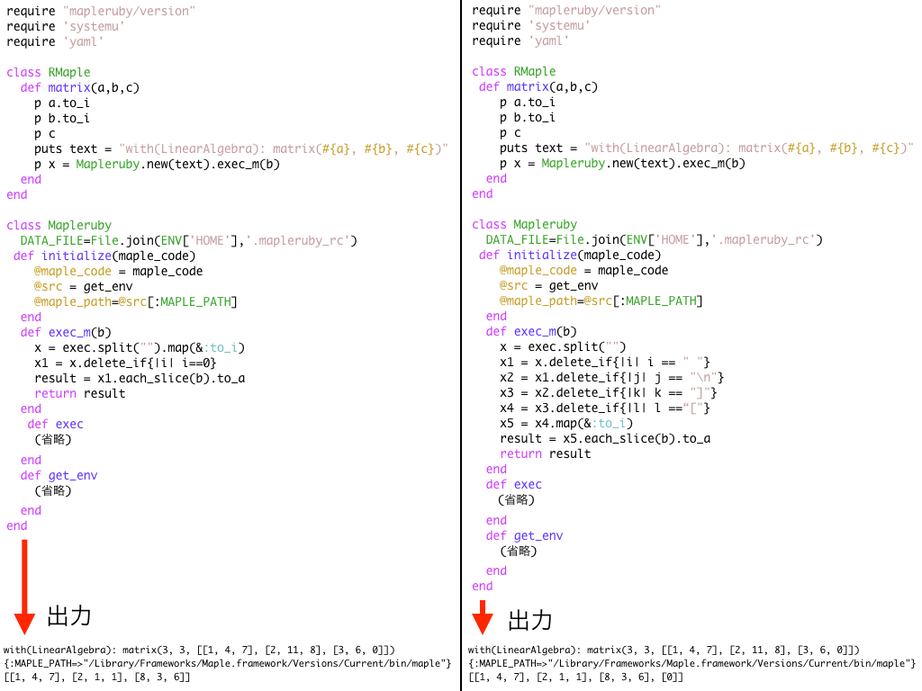
\includegraphics[width=10cm,bb= 0 0 737 553]{../figs/./mapleruby_eringi.005.png}
\caption{exec\_m(b)の完成形.}
\label{default}\end{center}\end{figure}
完成形では,まずgsubメソッドで数字以外の記号を空白に置き換え,splitメソッドで空白を指定することで空白を区切りとした配列にした後int型に直す.直した配列はその後,先ほどと同様にeach\_sliceメソッドを用いてlistlist構造になるようにしている.

\subsection{動的メソッドを用いての実装}
一通り実装した後,次に動的メソッドを用いて実装することにより重複コードを減らすように試みたバージョン2を作成した.

\begin{figure}[htbp]\begin{center}
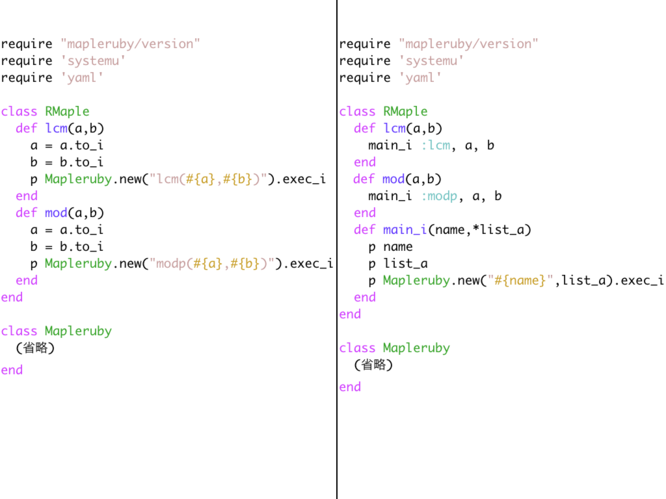
\includegraphics[width=10cm,bb= 0 0 737 553]{../figs/./mapleruby_eringi.006.png}
\caption{左が初期バージョン,右がバージョン2.}
\label{default}\end{center}\end{figure}
初期バージョンでは,関数ごとに各引数を好ましい型に変換した後Maplerubyクラスに遷移していた.
バージョン2では,各数学関数はMapleでの関数名と引数のみになり,新たに作ったmain\_i関数にそれらを送ることで初期バージョンと同様の動作を実装している.main\_i関数の第二引数が可変長引数になっているのは関数によって入力されている引数の個数が違うためである.例えばmain\_i関数は出力がint型である関数に対して使っており,図6のように実装した関数の重複部分や出力に応じて分類して,それぞれ関数を追加している.

\newpage

\begin{figure}[htbp]\begin{center}
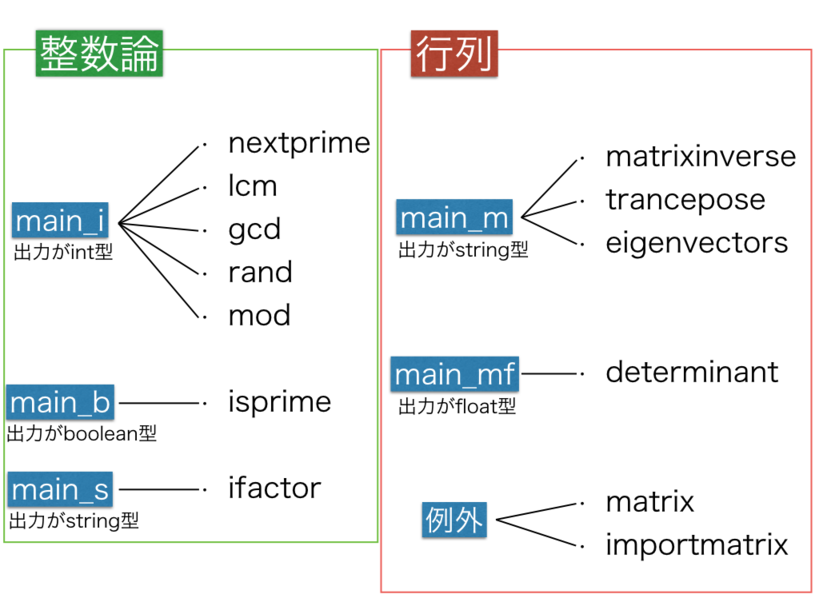
\includegraphics[width=10cm,bb= 0 0 737 553]{../figs/./mapleruby_eringi.007.png}
\caption{関数の分類.}
\label{default}\end{center}\end{figure}
matrixは他にexec\_m(b)を使う関数がないため,importmatrixは他と重複するコードがないため例外としている.


\section{検証}
\subsection{RSA暗号を用いた検証}
整数論に関する関数はRSA暗号の計算を用いて,Rubyのみで計算する場合とmaplerubyで計算した場合でどのような差があるか検証する.検証のために以下のようなプログラムを用意した.
\begin{lstlisting}[style=customRuby,basicstyle={\scriptsize\ttfamily}]
#rsa_org.rb
require 'prime'
include Math

def rsa(input)
  c = input.to_i
  print "平文>>> #{c}\n"
  
  big_num = sqrt(c).to_i
  num = 1000
  
  p,q,n=0,0,0
  p = Prime.each.find{|e| e >= rand(big_num+1..big_num+num)}
  q = Prime.each.find{|e| e >= rand(big_num+1..big_num+num)}
  
  n = p*q
  l = (p-1).lcm(q-1)
  
  print "素数 p >>> #{p}\n"
  print "素数 q >>> #{q}\n"
  print "N >>> #{n}\n"
  print "L >>> #{l}\n"
  
  for e in 2..l do
    break if e.gcd(l)==1
  end
  
  print "公開鍵>>> E = #{e}, N = #{n}\n"
  
  for d in 2..l do
    break if (e*d)%l==1
  end
  
  print "秘密鍵>>> D = #{d}, N = #{n}\n"
  
  m = c**e % n
  re_c = m**d % n
  
  print "暗号化>>> #{m}\n"
  print "復号化>>> #{re_c}\n"
end

rsa(ARGV[0])
\end{lstlisting}
このプログラムはRubyだけで書かれている.例えば平文を256と入力すると,
\begin{lstlisting}[style=,basicstyle={\scriptsize\ttfamily}]
/Users/eri/mapleruby/lib% ruby rsa.rb 256
平文>>> 256
素数 p >>> 107
素数 q >>> 83
N >>> 8881
L >>> 4346
公開鍵>>> E = 3, N = 8881
秘密鍵>>> D = 1449, N = 8881
暗号化>>> 1007
復号化>>> 256
\end{lstlisting}
このような形で,出力してくれる.

\subsubsection{RSA暗号とは}
RSA暗号は桁数が大きい合成数の素因数分解問題が困難であることを安全性の根拠とした公開鍵暗号の1つである.
1977年に発明され,発明者であるロナルド・リベスト(Ron Rivest),アディ・シャミア(Adi Shamir),
レオナルド・エーデルマン(Len Adleman)ら3人のFamily nameの頭文字をつなげてこのように呼ばれている\cite{listings2}.
アルゴリズムは,

\begin{itemize}
\item p, q: 任意の素数.
\item N: p, qをかけた数.
\item L: p - 1とq - 1の最小公倍数.
\item E(Encryption exponent, 暗号化指数): Lと互いに素な数.Lとの最大公約数が1となる数.
\item D(Decryption exponent, 復号化指数): E*D mod L = 1となる数.
\end{itemize}
以上6つの値を用いて,平文を暗号化していく.
ここでの数Eと数Nのペアが公開鍵,数Dと数Nのペアが秘密鍵となる.
平文を暗号化する際は,
\begin{quote}\begin{verbatim}
 平文^E mod N (平文をE乗してNで割った余り)
\end{verbatim}\end{quote}
を行い,逆に復号化する際は,
\begin{quote}\begin{verbatim}
 暗号文^D mod N (暗号文をD乗してNで割った余り)
\end{verbatim}\end{quote}
を行う.

\subsubsection{Rubyのみで計算した場合}
Rubyのみで計算した場合,このプログラムでは,平文が1000000を越えたあたりから正しく出力ができなかったり数が大きすぎて計算ができないということが起こる.下記は平文が2000000だった場合の結果である.
\begin{lstlisting}[style=,basicstyle={\scriptsize\ttfamily}]
/Users/eri/mapleruby/lib% ruby rsa_org.rb 2000000
平文>>> 2000000
素数 p >>> 1459
素数 q >>> 1493
N >>> 2178287
L >>> 1087668
公開鍵>>> E = 5, N = 2178287
秘密鍵>>> D = 652601, N = 2178287
rsa_org.rb:36: warning: in a**b, b may be too big
暗号化>>> 1481122
復号化>>> NaN
\end{lstlisting}
\subsubsection{maplerubyを使った場合}
まず先ほどのrsa\_org.rbをmaplerubyを用いたrsa.rbに書き換えた.
\begin{lstlisting}[style=customRuby,basicstyle={\scriptsize\ttfamily}]
#rsa.rb
require './mapleruby'
include Math

def rsa(input)
  c = input.to_i
  print "平文>>> #{c}\n"
  
  big_num = sqrt(c).to_i
  num = 1000
  
  p,q,n=0,0,0
  p = RMaple.new.nextprime(rand(big_num+1..big_num+num))
  q = RMaple.new.nextprime(rand(big_num+1..big_num+num))
  
  n = p*q
  l = RMaple.new.lcm(p-1,q-1)
  
  print "素数 p >>> #{p}\n"
  print "素数 q >>> #{q}\n"
  print "N >>> #{n}\n"
  print "L >>> #{l}\n"
  
  for e in 2..l do
    break if RMaple.new.gcd(e,l)==1
  end
  
  print "公開鍵>>> E = #{e}, N = #{n}\n"
  
  d = Mapleruby.new("eval(1/#{e} mod #{l})").exec_i
  
  print "秘密鍵>>> D = #{d}, N = #{n}\n"
  
  x = Mapleruby.new("#{c}^#{e}").exec_i
  m = RMaple.new.mod(x, n)
  
  re_c = Mapleruby.new("#{m}^#{d} mod #{n}").exec_i
  
  print "暗号化>>> #{m}\n"
  print "復号化>>> #{re_c}\n"
end

rsa(ARGV[0])
\end{lstlisting}
このプログラムに関しては,maplerubyのrand関数では乱数が同じ値になって計算がうまくいかなくなるためRubyのrand関数を使用している.
rsa.rbを使った場合は,1000000000までの暗号化が可能であると分かった.
\begin{lstlisting}[style=,basicstyle={\scriptsize\ttfamily}]
/Users/eri/mapleruby/lib% ruby rsa.rb 1000000000
平文>>> 1000000000
{:MAPLE_PATH=>"/Library/Frameworks/Maple.framework/Versions/Current/bin/maple"}
31699
{:MAPLE_PATH=>"/Library/Frameworks/Maple.framework/Versions/Current/bin/maple"}
31657
{:MAPLE_PATH=>"/Library/Frameworks/Maple.framework/Versions/Current/bin/maple"}
167238648
素数 p >>> 31699
素数 q >>> 31657
N >>> 1003495243
L >>> 167238648
{:MAPLE_PATH=>"/Library/Frameworks/Maple.framework/Versions/Current/bin/maple"}
2
{:MAPLE_PATH=>"/Library/Frameworks/Maple.framework/Versions/Current/bin/maple"}
3
{:MAPLE_PATH=>"/Library/Frameworks/Maple.framework/Versions/Current/bin/maple"}
4
{:MAPLE_PATH=>"/Library/Frameworks/Maple.framework/Versions/Current/bin/maple"}
1
公開鍵>>> E = 5, N = 1003495243
{:MAPLE_PATH=>"/Library/Frameworks/Maple.framework/Versions/Current/bin/maple"}
秘密鍵>>> D = 100343189, N = 1003495243
{:MAPLE_PATH=>"/Library/Frameworks/Maple.framework/Versions/Current/bin/maple"}
{:MAPLE_PATH=>"/Library/Frameworks/Maple.framework/Versions/Current/bin/maple"}
96903649
{:MAPLE_PATH=>"/Library/Frameworks/Maple.framework/Versions/Current/bin/maple"}
暗号化>>> 96903649
復号化>>> 1000000000
\end{lstlisting}\begin{description}
\item[MAPLE\_PATHの文章のところでmaplerubyが動いている.
]\end{description}
\subsection{行列での検証}
まず,以下のようなプログラムを作った.
\begin{lstlisting}[style=customRuby,basicstyle={\scriptsize\ttfamily}]
require './mapleruby'

a = 3
b = 3
c = [[1,2,1],[4,5,6],[7,8,9]]

p x = RMaple.new.matrix(a, b, c)

p RMaple.new.matrixinverse(x)
p RMaple.new.eigenvectors(x)
\end{lstlisting}
これは3行3列の行列を生成したのち,それの逆行列と固有値・固有ベクトルを出力するプログラムである.これを実行すると図9のようになる.

\begin{figure}[htbp]\begin{center}
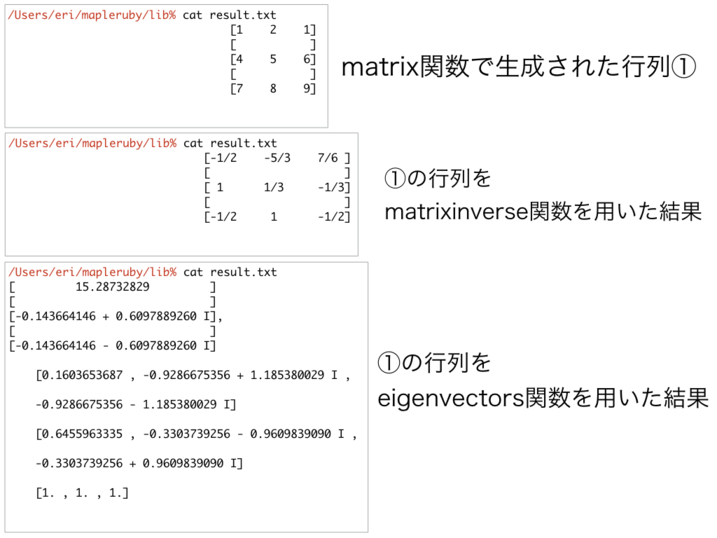
\includegraphics[width=10cm,bb= 0 0 737 553]{../figs/./mapleruby_eringi.008.png}
\caption{プログラムの出力結果}
\label{default}\end{center}\end{figure}
これと同じものをMapleで計算すると図10のようになる.

\begin{figure}[htbp]\begin{center}
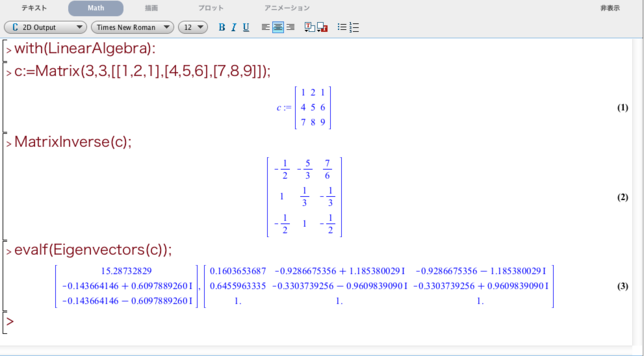
\includegraphics[width=10cm,bb= 0 0 737 553]{../figs/./mapleruby_eringi.exmaple.png}
\caption{Mapleの出力結果}
\label{default}\end{center}\end{figure}
よって正しく行列の計算ができた事が分かる.


\section{考察}
\subsection{初期バージョンとバージョン2の比較}
初期バージョンとバージョン2では,後者の方がプログラム自体の行数は多い.しかしそれは動的メソッドを実装するにあたって重複分をまとめた関数を増やしたためである.今後新たに数学関数を実装していくと仮定した場合,既に重複分がまとめてある関数を実装するならば,プログラムに書き足すのは実装する数学関数についての関数のみであるので,かなり簡潔で済む.
一方で,既に実装されているものと重複がないまたは出力が同じでない場合,初期バージョンと同じようにプログラムを書くことになる.加えて初期バージョンはMapleに送る式を必ず書くため,Mapleでのプログラムに慣れた人には初期バージョンの方で実装する方が容易かもしれない.

\begin{figure}[htbp]\begin{center}
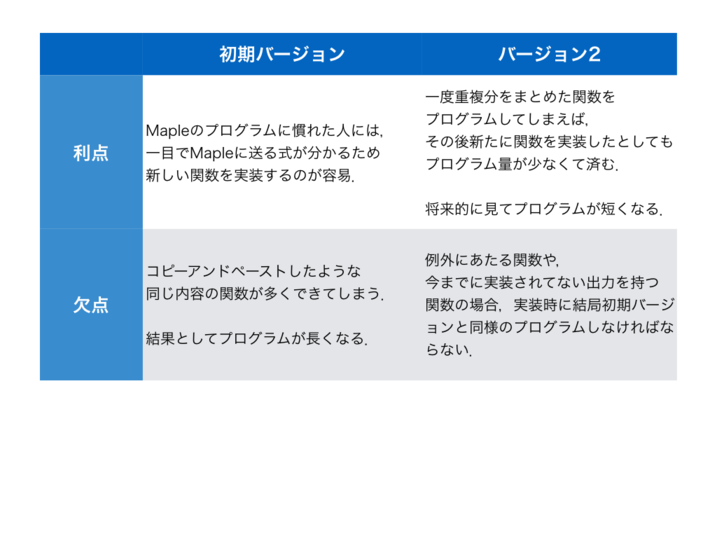
\includegraphics[width=12cm,bb= 0 0 937 753]{../figs/./mapleruby_eringi.009.png}
\caption{各バージョンの利点,欠点.}
\label{figure:eight}
\label{default}\end{center}\end{figure}
\subsection{maplerubyを使うメリット,デメリット}
最大のメリットは,Rubyだけで桁数の大きい計算や複雑な数学関数を必要とする計算を完結させられることである.今後扱える関数を増やせば,利用者がMapleについて詳しくない人でもRubyのプログラムを書くだけで数値計算処理が可能になるだろう.またRubyライブラリにあるTest::Unitと並行して使用すれば,求めたい解が分かっている際に自分が書いたプログラムで正しく解が導けるのかテストすることも可能である.

デメリットは大きく3つある.1つ目はRubyは無償で使えるがMapleは有償である点.よって,利用者が限られてしまう.2つ目はRMapleクラスの中に使いたい関数が実装されてない場合,自力で関数を実装するかMaplerubyクラスを直に使うかしなければならない点.よってプログラミングにMapleの知識が必要になってくるためメリットで挙げた「Rubyプログラムを書くだけで数値計算処理が可能になる」のが難しくなる.3つ目は桁数の大きい計算は確かにできるものの,処理に多少時間がかかってしまう点.処理速度を上げようと思うとMaple自体の処理速度を上げなければならない.


\section{おわりに}
\subsection{今後の課題}
\subsubsection{関数の充実化}
今回は限られた関数のみを選抜して実装したが,他にもたくさんの数学関数がMapleには用意されている.
RSA暗号のプログラムをmaplerubyで実装した際に直接Maplerubyクラスに送ることで対応した等式の解を出力するevalや累乗などの
頻繁に使われるであろう関数についてできるだけ対応させる.
他にも桁数が大きな数値はそもそもRubyの変数が扱いきれない場合も考えられるので,そこにうまく対処できるような関数が欲しい.

\subsubsection{グラフの描画}
Mapleが綺麗にグラフを描画できる数式処理ソフトウェアであることを利用して,maplerubyもグラフ描画に対応させる.
MapleはCUI版でのグラフがかなり見にくく,二次元ならまだしも三次元になると何が何だか分からないグラフになるため,
画像としてのグラフを出力できるような関数を実装する.


\begin{thebibliography}{99}
\bibitem{listings1}  「Maple(メイプル) とは」, サイバネット, \verb|http://www.cybernet.co.jp/maple/product/maple/about.html,| 2017/02/01アクセス.
\bibitem{listings2}  \verb|「RSA暗号」, Wikipedia, https://ja.wikipedia.org/wiki/RSA暗号, 2017/02/01 アクセス.|\end{thebibliography}

\end{document}
